\documentclass[a4paper,12]{article}
\usepackage{amsmath, amsfonts, amssymb, amsthm, bm, graphics, bbm, color}
\usepackage{graphicx}
\usepackage{subfigure}
\usepackage{mathtools}
\usepackage[table]{xcolor}
\usepackage{url}
\usepackage{mathabx}
\usepackage{cancel}

\usepackage{multicol}
\usepackage{float}
\usepackage{caption}
\usepackage{mathalfa}
\usepackage{hyperref}
\usepackage{afterpage}
\usepackage{multirow}
\usepackage[section]{placeins}

\captionsetup{font=footnotesize}
\captionsetup{width=\textwidth}
\DeclareMathAlphabet\mathbfcal{OMS}{cmsy}{b}{n}
\newtheorem{theorem}{Theorem}[section]
\newtheorem{lemma}[theorem]{Lemma}
\newtheorem{corollary}[theorem]{Corollary}
\newtheorem{proposition}[theorem]{Proposition}
\theoremstyle{definition}
\newtheorem{definition}[theorem]{Definition}
\newtheorem{example}[theorem]{Example}
\newtheorem{remark}[theorem]{Remark}


%center table entries
\newcolumntype{P}[1]{>{\centering\arraybackslash}p{#1}}


\newcommand\y{\cellcolor{gray!50}}

\newcommand\p{\cellcolor{gray!25}}

\makeatletter
\newcommand\makebig[2]{%
  \@xp\newcommand\@xp*\csname#1\endcsname{\bBigg@{#2}}%
  \@xp\newcommand\@xp*\csname#1l\endcsname{\@xp\mathopen\csname#1\endcsname}%
  \@xp\newcommand\@xp*\csname#1r\endcsname{\@xp\mathclose\csname#1\endcsname}%
}
\makeatother

\makebig{biggg} {3.0}
\makebig{Biggg} {3.5}
\makebig{bigggg}{4.0}
\makebig{Bigggg}{4.5}
\makebig{biggggg}{5.0}
\makebig{Biggggg}{5.5}
\makebig{bigggggg}{6.0}
\makebig{Bigggggg}{6.5}

\newcommand\bovermat[2]{%
    \makebox[0pt][l]{$\smash{\overbrace{\phantom{%
                    \begin{matrix}#2\end{matrix}}}^{\text{#1}}}$}#2}

\newcommand\bundermat[2]{%
    \makebox[0pt][l]{$\smash{\underbrace{\phantom{%
                    \begin{matrix}#2\end{matrix}}}_{\text{#1}}}$}#2}

\newcommand\partialphantom{\vphantom{\frac{\partial e_{P,M}}{\partial w_{1,1}}}}


\newcommand{\raisesym}[2]{\raisebox{0.5\depth}{$#1\Biggggg \}$}}

% redefine paper size
\setlength{\oddsidemargin}{0in}
\setlength{\textwidth}{6.4in}
\setlength{\topmargin}{-0.5in}
\setlength{\textheight}{9.9in}
\setlength{\headheight}{0in}

%slanted vector symbols
\renewcommand{\vec}[1]{\mbox{\boldmath$#1$}}
\newcommand{\vect}[1]{\boldsymbol{#1}}

%vertical d symbol for integrals
\newcommand{\dif}{\mathrm{d}}
\newcommand{\im}{\mathrm{i}}

\newcommand{\bbR}{\mathbb{R}}
\newcommand{\tr}{\mathrm{tr}}

\newcommand{\vvtheta}{{\bm {\vartheta}}}
\newcommand{\vvphi}{{\bm {\varphi}}}
\newcommand{\vtheta}{{\bm {\theta}}}


\DeclareMathOperator*{\esssup}{ess \, sup}

\begin{document}
\title{Angle measures for an MPT characterisation of a computed irregular polyhedron}
%\author{P.D. Ledger}
\date{22nd March 2024}
\maketitle
We consider an irregular polyhedron $B=B_1 \cup B_2$ with $B_1$ being an irregular tetrahedron with vertices
\begin{equation}\label{eqn:tet1}
{\bm v}_1 = \begin{bmatrix} 0 \\ 0 \\ 0 \end{bmatrix}, {\bm v}_2 = \begin{bmatrix} 7 \\ 0 \\ 0 \end{bmatrix}, {\bm v}_3 = \begin{bmatrix} 5.5 \\ 4.6 \\ 0 \end{bmatrix}, {\bm v}_4 = \begin{bmatrix} 3.3 \\ 2 \\ 5 \end{bmatrix},
\end{equation}
and $B_2$ the irregular tetrahedron with vertices
\begin{equation}
{\bm v}_1 = \begin{bmatrix} 0 \\ 0 \\ 0 \end{bmatrix}, {\bm v}_2 = \begin{bmatrix} 7 \\ 0 \\ 0 \end{bmatrix}, {\bm v}_3 = \begin{bmatrix} 5.5 \\ -3.0 \\ 0 \end{bmatrix}, {\bm v}_4 = \begin{bmatrix} 3.3 \\ 2 \\ 5 \end{bmatrix}
\end{equation}

\begin{figure}[h]
\begin{center}
$\begin{array}{cc}
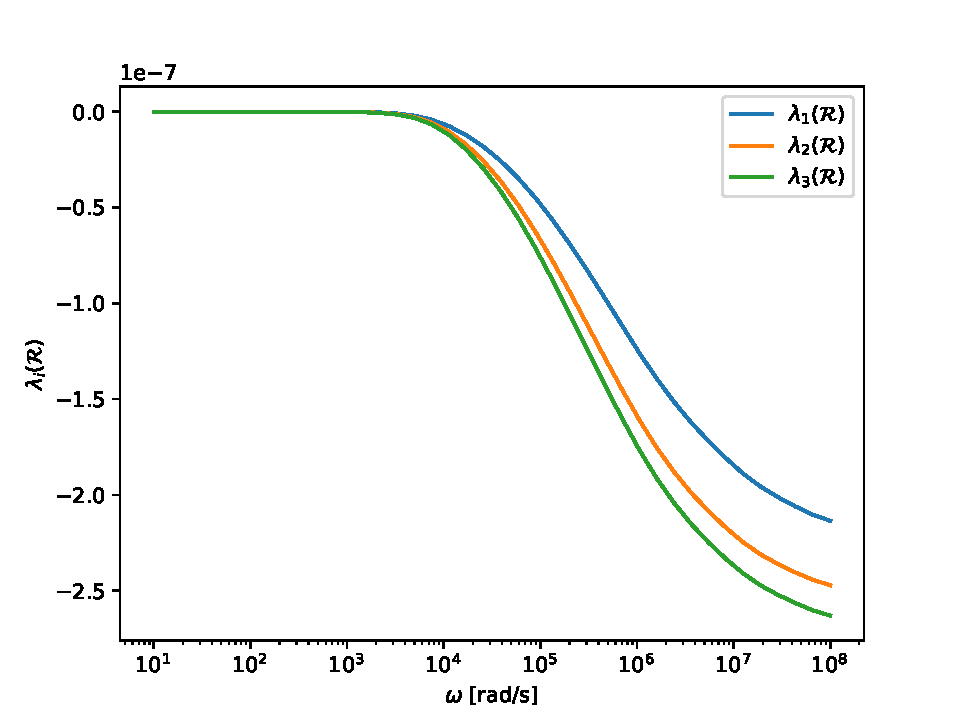
\includegraphics[width=0.5\textwidth]{CSG_TwoTetra_dRanddE__eig_R_al_0.001_mu_32_sig_1e7_ord3.pdf} &
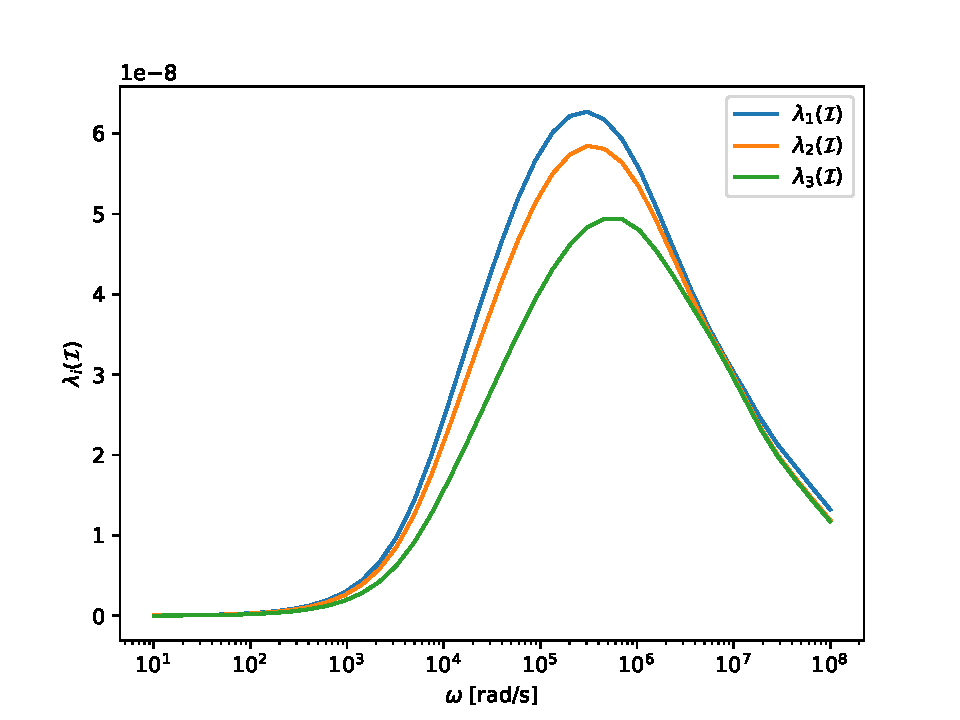
\includegraphics[width=0.5\textwidth]{CSG_TwoTetra_dRanddE__eig_I_al_0.001_mu_32_sig_1e7_ord3.pdf}
\\
\lambda_i({\mathcal R}) &\lambda_i({\mathcal I}) \\
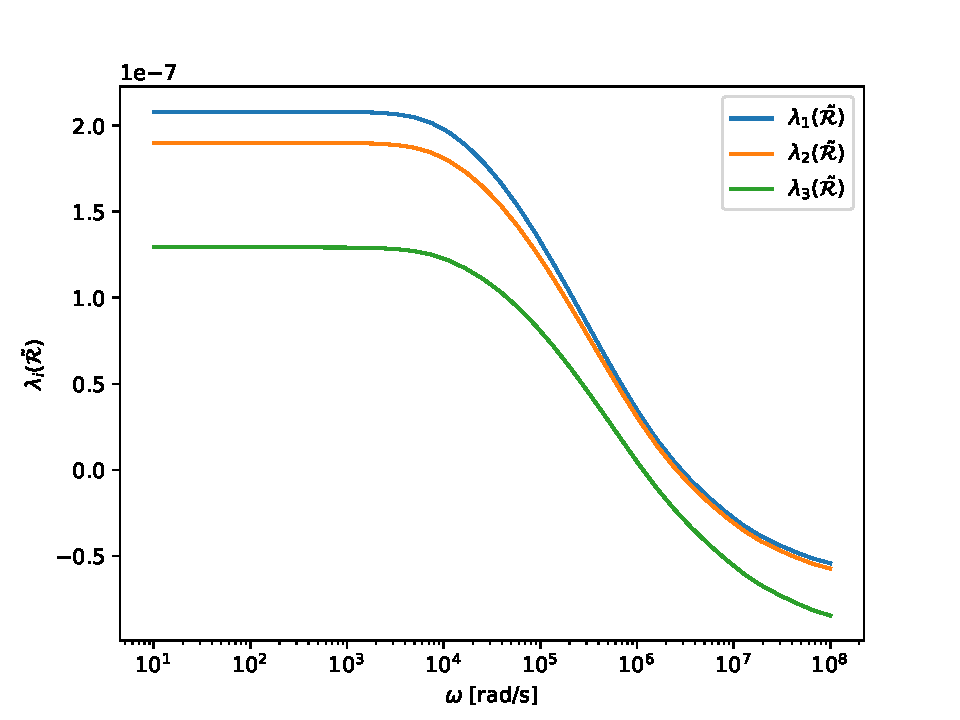
\includegraphics[width=0.5\textwidth]{CSG_TwoTetra_dRanddE__eig_Rtilde_al_0.001_mu_32_sig_1e7_ord3.pdf} &
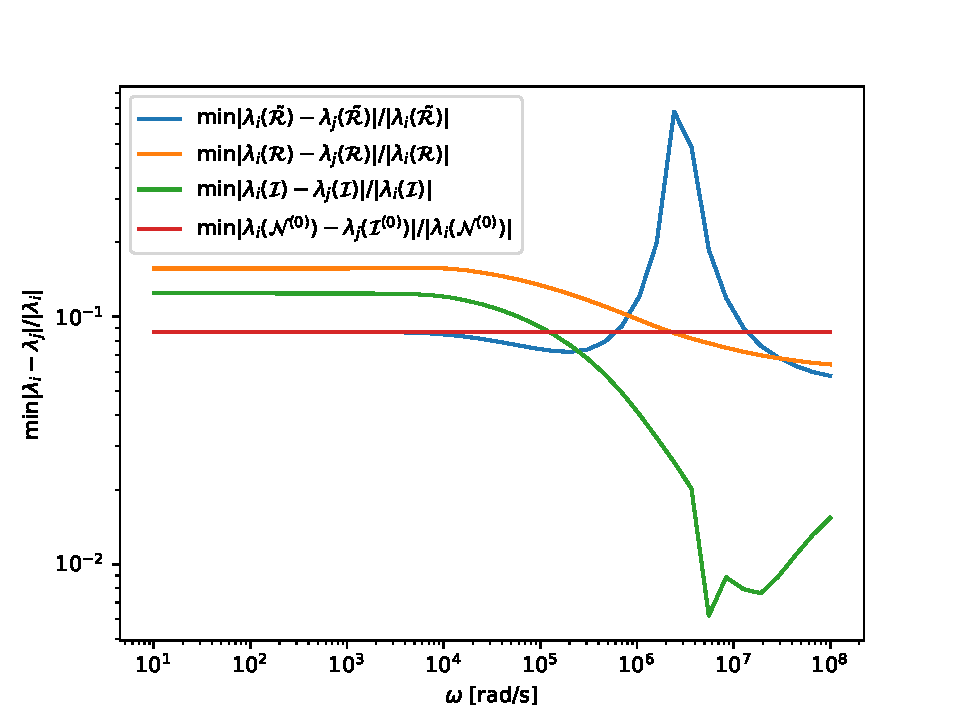
\includegraphics[width=0.5\textwidth]{CSG_TwoTetra_dRanddE__eig_prox_al_0.001_mu_32_sig_1e7_ord3.pdf} \\
\lambda_i(\tilde{\mathcal R}) & | \lambda_i -\lambda_j|/|\lambda_i| 
\end{array}$
\end{center}
\caption{Computed  eigenvalue spectral signatures and eigenvalue proximity an irregular polyhedron.}
\end{figure}
with $B_1\cap B_2 \ne \emptyset$ and $| B_1| > | B_2 |$. The object is chosen to have  $\alpha =0.001 $m and homogeneous materials $\mu_r = 32$ and $\sigma_*=1\times 10^7$ S/m.To discretise the object, $L=3$ layers of prismatic elements following the "geometric increasing" strategy are included resulting in a mesh consisting of 18\,413 unstructured tetrahedra and 6461 prisms.
\begin{figure}[h]
\begin{center}
$\begin{array}{cc}
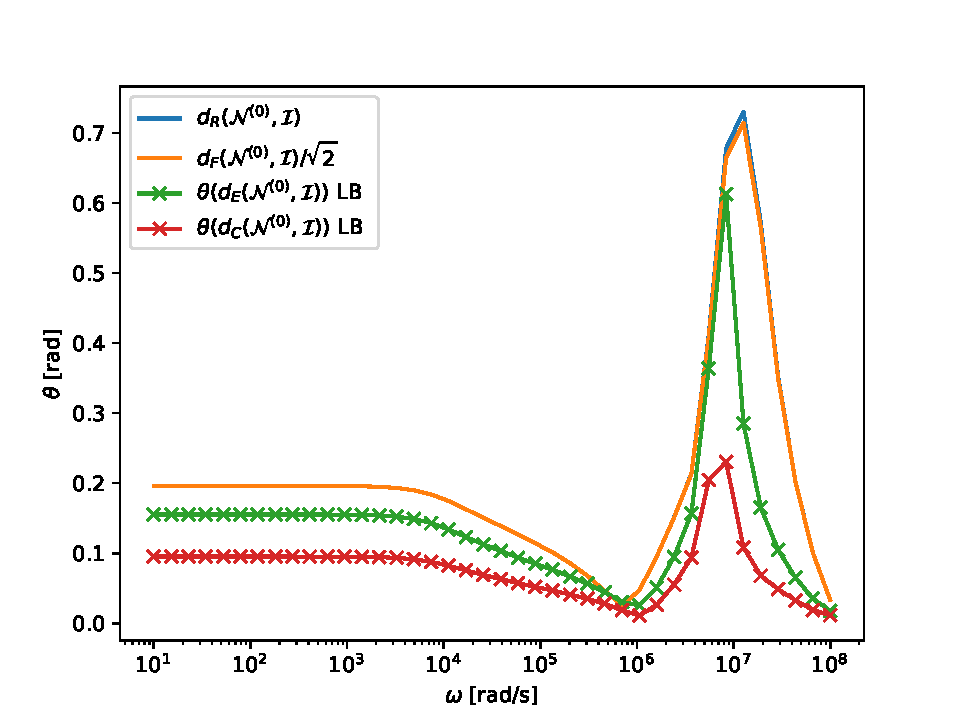
\includegraphics[width=0.5\textwidth]{CSG_TwoTetra_dRanddE_metrics_N0_al_0.001_mu_32_sig_1e7_ord3.pdf} &
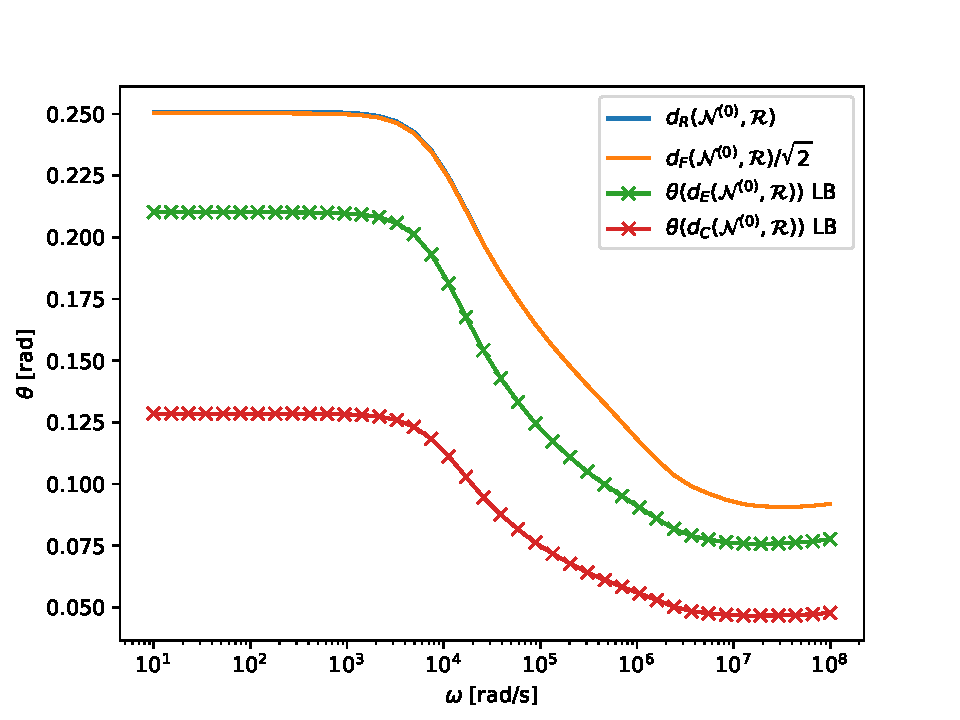
\includegraphics[width=0.5\textwidth]{CSG_TwoTetra_dRanddE_metrics_N0R_al_0.001_mu_32_sig_1e7_ord3.pdf} 
\end{array}$
\end{center}
\caption{Irregular polyhedron.  Left: Angle measures $d_R({\mathcal N}^{(0)}, {\mathcal I})$ and $d_F({\mathcal N}^{(0)}, {\mathcal I})/\sqrt{2}$ using the eigenvectors and $\theta(d_E({\mathcal N}^{(0)}, {\mathcal I}) $ and $\theta(d_C({\mathcal N}^{(0)}, {\mathcal I} ) $ without using the eigenvectors Right: Angle measures $d_R({\mathcal N}^{(0)}, {\mathcal R})$ and $d_F({\mathcal N}^{(0)}, {\mathcal R})/\sqrt{2}$ using the eigenvectors and $\theta(d_E({\mathcal N}^{(0)}, {\mathcal R}) $ and $\theta(d_C({\mathcal N}^{(0)}, {\mathcal R} ) $ without using the eigenvectors}
\end{figure}

\begin{figure}[h]
\begin{center}
$\begin{array}{cc}
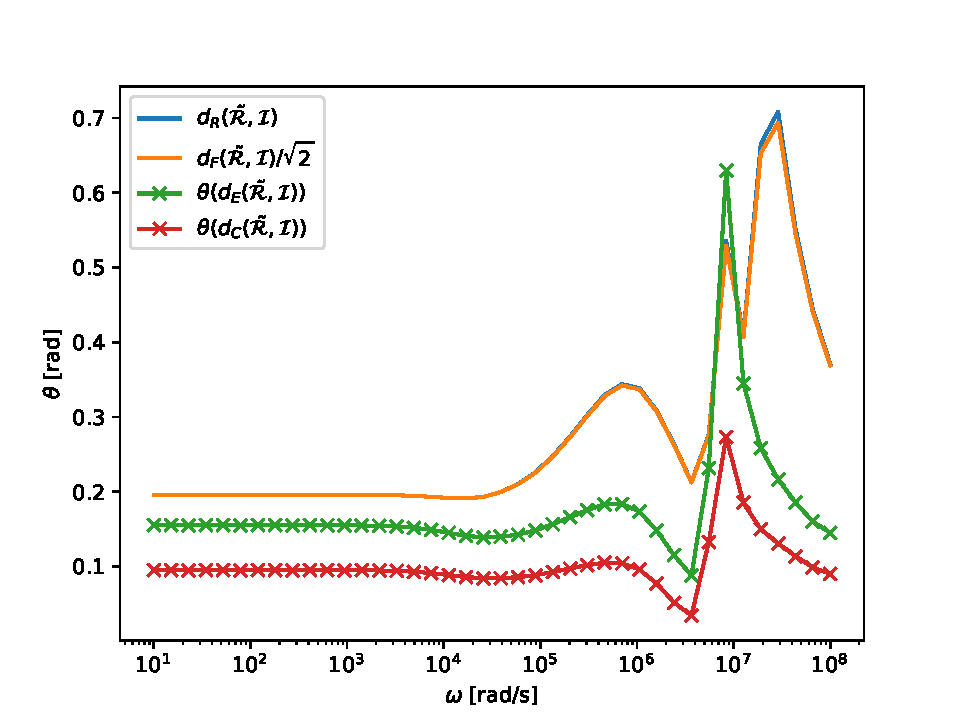
\includegraphics[width=0.5\textwidth]{CSG_TwoTetra_dRanddE_metrics_RtildeI_al_0.001_mu_32_sig_1e7_ord3.pdf} &
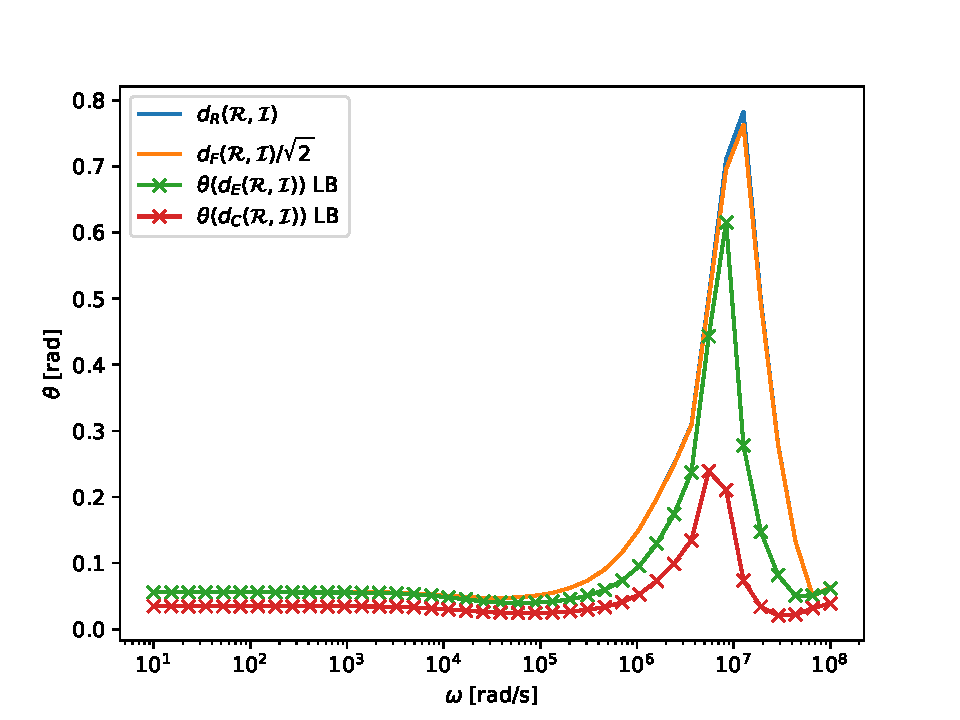
\includegraphics[width=0.5\textwidth]{CSG_TwoTetra_dRanddE_metrics_RI_al_0.001_mu_32_sig_1e7_ord3.pdf}\end{array}$
\end{center}
\caption{Irregular polyhedron.  Left:Angle measures $d_R(\tilde{\mathcal R}, {\mathcal I})$ and $d_F(\tilde{\mathcal R}, {\mathcal I})/\sqrt{2}$ using the eigenvectors and $\theta(d_E(\tilde{\mathcal R}, {\mathcal I}) $ and $\theta(d_C(\tilde{\mathcal R} , {\mathcal I} ) $ without using the eigenvectors. Right:$d_R({\mathcal R}, {\mathcal I})$ and $d_F({\mathcal R}, {\mathcal I})/\sqrt{2}$ using the eigenvectors and $\theta(d_E({\mathcal R}, {\mathcal I}) $ and $\theta(d_C({\mathcal R} , {\mathcal I} ) $ without using the eigenvectors 
}
\end{figure}

\end{document}
